% Options for packages loaded elsewhere
\PassOptionsToPackage{unicode}{hyperref}
\PassOptionsToPackage{hyphens}{url}
\documentclass[
  ignorenonframetext,
  aspectratio=169]{beamer}
\newif\ifbibliography
\usepackage{pgfpages}
\setbeamertemplate{caption}[numbered]
\setbeamertemplate{caption label separator}{: }
\setbeamercolor{caption name}{fg=normal text.fg}
\beamertemplatenavigationsymbolsempty
% remove section numbering
\setbeamertemplate{part page}{
  \centering
  \begin{beamercolorbox}[sep=16pt,center]{part title}
    \usebeamerfont{part title}\insertpart\par
  \end{beamercolorbox}
}
\setbeamertemplate{section page}{
  \centering
  \begin{beamercolorbox}[sep=12pt,center]{section title}
    \usebeamerfont{section title}\insertsection\par
  \end{beamercolorbox}
}
\setbeamertemplate{subsection page}{
  \centering
  \begin{beamercolorbox}[sep=8pt,center]{subsection title}
    \usebeamerfont{subsection title}\insertsubsection\par
  \end{beamercolorbox}
}
% Prevent slide breaks in the middle of a paragraph
\widowpenalties 1 10000
\raggedbottom
\AtBeginPart{
  \frame{\partpage}
}
\AtBeginSection{
  \ifbibliography
  \else
    \frame{\sectionpage}
  \fi
}
\AtBeginSubsection{
  \frame{\subsectionpage}
}
\usepackage{iftex}
\ifPDFTeX
  \usepackage[T1]{fontenc}
  \usepackage[utf8]{inputenc}
  \usepackage{textcomp} % provide euro and other symbols
\else % if luatex or xetex
  \usepackage{unicode-math} % this also loads fontspec
  \defaultfontfeatures{Scale=MatchLowercase}
  \defaultfontfeatures[\rmfamily]{Ligatures=TeX,Scale=1}
\fi
\usepackage{lmodern}
\ifPDFTeX\else
  % xetex/luatex font selection
\fi
% Use upquote if available, for straight quotes in verbatim environments
\IfFileExists{upquote.sty}{\usepackage{upquote}}{}
\IfFileExists{microtype.sty}{% use microtype if available
  \usepackage[]{microtype}
  \UseMicrotypeSet[protrusion]{basicmath} % disable protrusion for tt fonts
}{}
\makeatletter
\@ifundefined{KOMAClassName}{% if non-KOMA class
  \IfFileExists{parskip.sty}{%
    \usepackage{parskip}
  }{% else
    \setlength{\parindent}{0pt}
    \setlength{\parskip}{6pt plus 2pt minus 1pt}}
}{% if KOMA class
  \KOMAoptions{parskip=half}}
\makeatother
\usepackage{longtable,booktabs,array}
\usepackage{calc} % for calculating minipage widths
\usepackage{caption}
% Make caption package work with longtable
\makeatletter
\def\fnum@table{\tablename~\thetable}
\makeatother
\setlength{\emergencystretch}{3em} % prevent overfull lines
\providecommand{\tightlist}{%
  \setlength{\itemsep}{0pt}\setlength{\parskip}{0pt}}
% ============================================================
%  beamer_preamble.tex  (DEFAULT Beamer look + colored boxes)
%  - Keeps your font choices (Calibri) and scenario palette
%  - Restores default Beamer colors (no UW purple background, no white titles)
%  - Keeps colored blocks + scenario highlight macro + colored bullets
% ============================================================

% ── Beamer theme (keep default look) ─────────────────────────────────────────
\usetheme{default}
\usecolortheme{default}
\usefonttheme{professionalfonts}

% ── XeLaTeX fonts (requires xelatex engine) ─────────────────────────────────
\usepackage{fontspec}
\setmainfont{Calibri}[
  BoldFont       = Calibri Bold,
  ItalicFont     = Calibri Italic,
  BoldItalicFont = Calibri Bold Italic
]
\setsansfont{Calibri}
\setmonofont{Courier New}

% ── Packages ────────────────────────────────────────────────────────────────
\usepackage{booktabs}
\usepackage{xcolor}
\usepackage{soul}          % for \hl highlighting
\usepackage{colortbl}
\usepackage{array}
\usepackage{graphicx}
\usepackage{ragged2e}
\usepackage{microtype}
\usepackage{hyperref}

% ── Project colour palette (definitions only) ───────────────────────────────
% Keep UW colors defined (useful for occasional accents), but we do NOT apply
% them globally to titles/backgrounds.
\definecolor{uwpurple}{HTML}{4B2E83}      % UW brand purple (defined, not global)
\definecolor{uwgold}{HTML}{85754D}        % UW brand gold  (defined, not global)

% Scenario / figure colors
\definecolor{ambitiousblue}{HTML}{2171B5} % headline scenario
\definecolor{progressgreen}{HTML}{74C476}
\definecolor{aspirationalpurple}{HTML}{6A3D9A}
\definecolor{baugrey}{HTML}{999999}
\definecolor{highlightblue}{HTML}{DBEAFE} % table row highlight

% ── HARD RESET: ensure default Beamer colors (no purple canvas / white titles)
% These lines intentionally avoid overriding Beamer's defaults.
% Reset structure color to default black
\setbeamercolor{structure}{fg=black}

% Ensure title elements are black
\setbeamercolor{title}{fg=black}
\setbeamercolor{subtitle}{fg=black}
\setbeamercolor{author}{fg=black}
\setbeamercolor{date}{fg=black}
\setbeamercolor{institute}{fg=black}
\setbeamercolor{frametitle}{fg=black}
\setbeamercolor{normal text}{fg=black}

% IMPORTANT: do NOT set a custom background template (keeps default)
% \setbeamertemplate{background}{...}     % intentionally NOT used

% IMPORTANT: do NOT override the frametitle template (keeps default)
% \setbeamertemplate{frametitle}{...}     % intentionally NOT used

% ── Colored blocks (boxes) ──────────────────────────────────────────────────
% Default "block" = neutral/BAU-style
\setbeamercolor{block title}{bg=baugrey!15, fg=black}
\setbeamercolor{block body}{bg=baugrey!6}

% Alert blocks = red
\setbeamercolor{block title alerted}{bg=red!15, fg=red!70!black}
\setbeamercolor{block body alerted}{bg=red!6}

% Example blocks = ambitious blue
\setbeamercolor{block title example}{bg=ambitiousblue!15, fg=ambitiousblue!85!black}
\setbeamercolor{block body example}{bg=ambitiousblue!6}

% Optional: custom block environments for Progress / Aspirational
\newenvironment{progressblock}[1]{%
  \setbeamercolor{block title}{bg=progressgreen!18, fg=progressgreen!80!black}%
  \setbeamercolor{block body}{bg=progressgreen!6}%
  \begin{block}{#1}%
}{\end{block}}

\newenvironment{aspirationalblock}[1]{%
  \setbeamercolor{block title}{bg=aspirationalpurple!15, fg=aspirationalpurple!80!black}%
  \setbeamercolor{block body}{bg=aspirationalpurple!5}%
  \begin{block}{#1}%
}{\end{block}}

\newenvironment{baublock}[1]{%
  \setbeamercolor{block title}{bg=baugrey!18, fg=black}%
  \setbeamercolor{block body}{bg=baugrey!6}%
  \begin{block}{#1}%
}{\end{block}}

% ── Bullet style (accent without changing global theme) ─────────────────────
\setbeamertemplate{itemize item}{\textcolor{ambitiousblue}{\textbullet}}
\setbeamertemplate{itemize subitem}{\textcolor{ambitiousblue}{--}}
\setbeamertemplate{enumerate item}{\textcolor{ambitiousblue}{\insertenumlabel.}}

% ── Headline scenario highlight command ─────────────────────────────────────
% \hlambitious{text} -- blue-boxed highlight for the Ambitious scenario
\newcommand{\hlambitious}[1]{%
  \colorbox{ambitiousblue!20}{\textcolor{ambitiousblue}{\textbf{#1}}}%
}

% ── Optional: keep a clean footer (NOT purple background) ───────────────────
% Comment out this entire block if you want Beamer's default footer.
\setbeamertemplate{footline}{%
  \leavevmode
  \hbox{%
    \begin{beamercolorbox}[wd=0.45\paperwidth, ht=2.25ex, dp=1ex, left]{author in head/foot}%
      \hspace{1em}\usebeamerfont{author in head/foot}%
      \textcolor{black!60}{\footnotesize WHO -- UW CVD Targets 2030}%
    \end{beamercolorbox}%
    \begin{beamercolorbox}[wd=0.45\paperwidth, ht=2.25ex, dp=1ex, center]{title in head/foot}%
      \usebeamerfont{title in head/foot}%
      \textcolor{black!60}{\footnotesize Aim 1: Modelling Study}%
    \end{beamercolorbox}%
    \begin{beamercolorbox}[wd=0.10\paperwidth, ht=2.25ex, dp=1ex, right]{date in head/foot}%
      \usebeamerfont{date in head/foot}%
      \textcolor{black!60}{\footnotesize \insertframenumber{}/\inserttotalframenumber}%
      \hspace{0.5em}%
    \end{beamercolorbox}%
  }%
  \vskip0pt%
}
\setbeamertemplate{navigation symbols}{}

% ── Section slide (auto-generated by # headers) ─────────────────────────────
% Keeps default look (no purple canvas); uses a subtle neutral box.
\AtBeginSection[]{%
  \begin{frame}
    \vfill
    \centering
    \begin{beamercolorbox}[sep=8pt, center, shadow=false, rounded=true]{block title}
      \usebeamerfont{title}\insertsectionhead\par
    \end{beamercolorbox}
    \vfill
  \end{frame}
}
\usepackage{booktabs}
\usepackage{longtable}
\usepackage{array}
\usepackage{multirow}
\usepackage{wrapfig}
\usepackage{float}
\usepackage{colortbl}
\usepackage{pdflscape}
\usepackage{tabu}
\usepackage{threeparttable}
\usepackage{threeparttablex}
\usepackage[normalem]{ulem}
\usepackage{makecell}
\usepackage{xcolor}
\usepackage{bookmark}
\IfFileExists{xurl.sty}{\usepackage{xurl}}{} % add URL line breaks if available
\urlstyle{same}
\hypersetup{
  pdftitle={Projected Health Impact of Achieving WHO Targets for Cardiovascular Risk-Factor Control},
  pdfauthor={Work in Progress},
  hidelinks,
  pdfcreator={LaTeX via pandoc}}

\title{Projected Health Impact of Achieving WHO Targets for
Cardiovascular Risk-Factor Control}
\author{\color{blue}Work in Progress}
\date{August 2026}
\institute{WHO \(\cdot\) University of Washington}

\begin{document}
\frame{\titlepage}

\begin{frame}[allowframebreaks]
  \setcounter{tocdepth}{3}
  \tableofcontents
\end{frame}
\setcounter{tocdepth}{3}
\tableofcontents
}
\begin{frame}
\end{frame}

\section{Study Overview}\label{study-overview}

\begin{frame}{Aim 1: Research Questions}
\phantomsection\label{aim-1-research-questions}
\begin{block}{Central Question}
What is the projected \textbf{burden-of-disease impact} of achieving the WHO cardiovascular risk-factor control targets by \textbf{2030}?
\end{block}

\textbf{Sub-questions driving the analysis:}

\begin{enumerate}
  \item How many \textbf{cardiovascular events} could be averted?
  
  \item How many \textbf{CVD deaths} could be prevented by 2030 and beyond?
  
  \item How would \textbf{life-years, YLLs, YLDs, and DALYs} change under joint achievement of:
  \begin{itemize}
      \item 150M additional people with controlled hypertension
      \item $\geq$50\% lipid-lowering therapy coverage
      \item 80\% BP control among people with diabetes
      \item \alert{80\% validated BP device availability}
  \end{itemize}
\end{enumerate}

\medskip
\begin{columns}[T]

\begin{column}{0.48\textwidth}
\begin{exampleblock}{Scope}
\small
\textbf{186 countries} $\cdot$ Ages 20--95 $\cdot$ 2026--2050 $\cdot$ Multiple CVD causes $\cdot$ WHO Target Scenarios
\end{exampleblock}
\end{column}

\begin{column}{0.48\textwidth}
\begin{alertblock}{Intervention start: 2026}
\small
Model calibrated to 2019 baseline. First year of target scale-up effects entering the projection is \textbf{2026}.
\end{alertblock}
\end{column}

\end{columns}
\end{frame}

\begin{frame}{Study Design at a Glance}
\phantomsection\label{study-design-at-a-glance}
\begin{table}[!h]
\centering\begingroup\fontsize{8}{10}\selectfont

\begin{tabular}{>{\raggedright\arraybackslash}p{3.2cm}>{\raggedright\arraybackslash}p{9.8cm}}
\toprule
Component & Detail\\
\midrule
\textbf{\cellcolor{gray!10}{Model type}} & \cellcolor{gray!10}{Discrete-time multi-state model (Well $\to$ Sick $\to$ Dead)}\\
\textbf{Calibration data} & GBD 2023: incidence, case fatality, prevalence; all-cause \& CVD-specific\\
\textbf{\cellcolor{gray!10}{Population data}} & \cellcolor{gray!10}{UNWPP 2024 single-year age/sex projections}\\
\cellcolor[HTML]{dbeafe}{\textbf{Intervention start}} & \cellcolor[HTML]{dbeafe}{\textbf{2026} --- first year intervention effects enter the projection}\\
\textbf{\cellcolor{gray!10}{Scale-up period}} & \cellcolor{gray!10}{Linear scale-up 2026 $\to$ 2030; rates held constant 2030--2050}\\
\addlinespace
\textbf{Comparison} & Business-as-usual: 2024 control rates, no additional scale-up\\
\textbf{\cellcolor{gray!10}{Outcome}} & \cellcolor{gray!10}{CVD deaths averted vs.~BAU; age-standardised mortality rate (ASMR)}\\
\textbf{Time horizon} & 2026--2050 (25-year horizon); model calibrated from 2019\\
\bottomrule
\end{tabular}
\endgroup{}
\end{table}
\end{frame}

\begin{frame}{Study Context}
\phantomsection\label{study-context}
\begin{columns}[T]
\begin{column}{0.55\textwidth}
\textbf{Objective}
\begin{itemize}
  \item Quantify CVD deaths avertable by achieving WHO 2030 cardiovascular targets
  \item Coverage: \textbf{186 countries}, 2025–2050
  \item Four causes: IHD, ischemic stroke, hemorrhagic stroke, hypertensive HD
\end{itemize}
\vspace{6pt}
\textbf{Model}
\begin{itemize}
  \item Discrete-time state transition (Well $\to$ Sick $\to$ Dead)
  \item Calibrated to GBD 2023; projected with UNWPP 2024 populations
  \item 8 blood-pressure bins
  \item Baseline treatment effects explicitly de-duplicated
\end{itemize}
\end{column}
\begin{column}{0.43\textwidth}
\begin{exampleblock}{Research Question}
What are the projected deaths averted from achieving WHO hypertension control and lipid-lowering therapy targets across \textbf{186 countries}, 2026--2050?
\end{exampleblock}
\begin{block}{Pending \textcolor{red!70!black}{$\bigtriangleup$}}
Confirm primary metric: deaths averted vs.\ DALYs vs.\ LYG
\end{block}
\end{column}
\end{columns}
\end{frame}

\section{Data Sources}\label{data-sources}

\begin{frame}{Data Sources and Key Variables}
\phantomsection\label{data-sources-and-key-variables}
\begin{table}[!h]
\centering\begingroup\fontsize{8}{10}\selectfont

\begin{tabular}{>{\raggedright\arraybackslash}p{2.8cm}>{\raggedright\arraybackslash}p{6.8cm}>{\raggedright\arraybackslash}p{3.4cm}}
\toprule
Source & Variables extracted & Role in model\\
\midrule
\textbf{\cellcolor{gray!10}{GBD 2023 (IHME)}} & \cellcolor{gray!10}{IR, CF, prevalence, background mortality (age/sex/country)} & \cellcolor{gray!10}{Baseline transition rates; initial states}\\
\textbf{GBD 2019 (IHME)} & Relative risks per 10 mmHg SBP increase (IHD, stroke, HHD, by age) & Anchor BP-bin incidence; normalisation factor $\alpha$\\
\textbf{\cellcolor{gray!10}{Ettehad et al.\ 2016}} & \cellcolor{gray!10}{Trial effect sizes per BP category; diabetes-stratified} & \cellcolor{gray!10}{Treatment effect sizes by BP bin $\times$ cause}\\
\textbf{UNWPP 2024 (UN)} & Population projections 2019--2050 (single-year age, sex, country) & Cohort sizes; rate denominators\\
\textbf{\cellcolor{gray!10}{NCD-RisC}} & \cellcolor{gray!10}{Baseline HTN control rates ($C_0$); BP distribution by country} & \cellcolor{gray!10}{$C_0$; $P(\text{BP}_{\text{cat}})$}\\
\addlinespace
\textbf{Country-specific} & HTN control targets 2030 (Progress / Ambitious / Aspirational) & $C_{\text{target}}$ per scenario\\
\bottomrule
\end{tabular}
\endgroup{}
\end{table}
\end{frame}

\section{Scenarios}\label{scenarios}

\begin{frame}{Four WHO Priority Targets}
\phantomsection\label{four-who-priority-targets}
\begin{table}[!h]
\centering\begingroup\fontsize{7}{9}\selectfont

\resizebox{\ifdim\width>\linewidth\linewidth\else\width\fi}{!}{
\begin{tabular}{r>{\raggedright\arraybackslash}p{4.5cm}>{\raggedright\arraybackslash}p{5.5cm}}
\toprule
\# & WHO Target & Modelled Scenario\\
\midrule
1 & 150M more with HTN controlled by 2030 & \textbf{HTN Control (Combined)}: 150.0M more controlled = 83.8M without + 66.2M with diabetes (mutually exclusive, additive)\\
2 & $\geq$50\% eligible adults on lipid-lowering therapy by 2030 & \textbf{Improved Statin Uptake}: 50\% coverage by 2030\\
3 & 80\% BP control among diagnosed diabetics by 2030 & \textbf{HTN Control (Diabetes)}: 0.80 aspirational ceiling by 2030 (66.2M of the 150M)\\
4 & 80\% availability of validated BP devices & Operationally embedded in HTN scenarios (150M Target [1+3])\\
\bottomrule
\end{tabular}}
\endgroup{}
\end{table}

\vspace{4pt}

\textbf{Combination rule:} the two BP subgroups combine
\emph{additively} as a population mixture,
\(\varepsilon_{IR,\text{BP}} = 1-(1-w_D)e_N - w_D e_D\); the BP
composite then combines multiplicatively with statins,
\(\varepsilon_{IR,\text{total}} = \varepsilon_{IR,\text{BP}} \times \varepsilon_{IR,\text{statin}}\).
\end{frame}

\begin{frame}{The 150 Million Target --- Additional BP Control by Region
and Diabetes Status}
\phantomsection\label{the-150-million-target-additional-bp-control-by-region-and-diabetes-status}
\begin{center}\includegraphics[width=\linewidth]{aim1_executive_slides_files/figure-beamer/scenario-split-plot-1} \end{center}
\end{frame}

\begin{frame}{HTN Control Target: 150 Million by WHO Region}
\phantomsection\label{htn-control-target-150-million-by-who-region}
\begin{table}[!h]
\centering\begingroup\fontsize{7}{9}\selectfont

\resizebox{\ifdim\width>\linewidth\linewidth\else\width\fi}{!}{
\begin{tabular}{lrrrrrrr}
\toprule
\textbf{Region} & \textbf{HTN pop 2025 (M)} & \textbf{Controlled 2025 (M)} & \textbf{Cov.\ 2025} & \textbf{Controlled 2030 (M)} & \textbf{Cov.\ 2030} & \textbf{Added (M)} & \textbf{+\%}\\
\midrule
Africa & 182.0 & 20.6 & 11.3\% & 29.1 & 16.0\% & 8.5 & 41.5\%\\
Americas & 273.9 & 100.4 & 36.7\% & 140.5 & 51.3\% & 40.1 & 40.0\%\\
Eastern Mediterranean & 157.5 & 24.0 & 15.2\% & 34.0 & 21.6\% & 10.0 & 41.5\%\\
Europe & 300.3 & 80.5 & 26.8\% & 113.9 & 37.9\% & 33.3 & 41.4\%\\
South-East Asia & 425.8 & 57.3 & 13.4\% & 81.1 & 19.0\% & 23.8 & 41.5\%\\
\addlinespace
Western Pacific & 456.1 & 83.5 & 18.3\% & 117.7 & 25.8\% & 34.2 & 41.0\%\\
\cellcolor[HTML]{2166ac}{\textcolor{white}{\textbf{Global}}} & \cellcolor[HTML]{2166ac}{\textcolor{white}{\textbf{1,795.5}}} & \cellcolor[HTML]{2166ac}{\textcolor{white}{\textbf{366.2}}} & \cellcolor[HTML]{2166ac}{\textcolor{white}{\textbf{20.4\%}}} & \cellcolor[HTML]{2166ac}{\textcolor{white}{\textbf{516.2}}} & \cellcolor[HTML]{2166ac}{\textcolor{white}{\textbf{28.8\%}}} & \cellcolor[HTML]{2166ac}{\textcolor{white}{\textbf{150.0}}} & \cellcolor[HTML]{2166ac}{\textcolor{white}{\textbf{41.0\%}}}\\
\bottomrule
\end{tabular}}
\endgroup{}
\end{table}

\footnotesize Coverage rates and 2030 counts use the fixed 2025
hypertensive population; regional additions sum to exactly 150 million.
\end{frame}

\begin{frame}{HTN Control Target: 150 Million by WHO Region \emph{and}
Diabetes Subgroup}
\phantomsection\label{htn-control-target-150-million-by-who-region-diabetes-subgroup}
\begin{table}[!h]
\centering\begingroup\fontsize{8}{10}\selectfont

\resizebox{\ifdim\width>\linewidth\linewidth\else\width\fi}{!}{
\begin{tabular}{lrrrrr}
\toprule
\multicolumn{1}{c}{\textbf{ }} & \multicolumn{3}{c}{\textbf{Additional controlled 2030 (M)}} & \multicolumn{2}{c}{\textbf{ }} \\
\cmidrule(l{3pt}r{3pt}){2-4}
\textbf{Region} & \textbf{No diabetes} & \textbf{Diabetes} & \textbf{Total} & \textbf{Cov.\ 2030} & \textbf{+\%}\\
\midrule
Africa & 4.3 & 4.3 & 8.5 & 16.0\% & 41.5\%\\
Americas & 24.7 & 15.5 & 40.1 & 51.3\% & 40.0\%\\
Eastern Mediterranean & 5.1 & 4.9 & 10.0 & 21.6\% & 41.5\%\\
Europe & 17.9 & 15.4 & 33.3 & 37.9\% & 41.4\%\\
South-East Asia & 12.3 & 11.5 & 23.8 & 19.0\% & 41.5\%\\
\addlinespace
Western Pacific & 19.5 & 14.7 & 34.2 & 25.8\% & 41.0\%\\
\cellcolor[HTML]{2166ac}{\textcolor{white}{\textbf{Global}}} & \cellcolor[HTML]{2166ac}{\textcolor{white}{\textbf{83.8}}} & \cellcolor[HTML]{2166ac}{\textcolor{white}{\textbf{66.2}}} & \cellcolor[HTML]{2166ac}{\textcolor{white}{\textbf{150.0}}} & \cellcolor[HTML]{2166ac}{\textcolor{white}{\textbf{28.8\%}}} & \cellcolor[HTML]{2166ac}{\textcolor{white}{\textbf{41.0\%}}}\\
\bottomrule
\end{tabular}}
\endgroup{}
\end{table}

\footnotesize Additional people with BP control by 2030, disaggregated
by WHO region \emph{and} mutually exclusive diabetes status (fixed 2025
population). Both the regional totals and the two subgroup totals sum to
exactly 150 million.
\end{frame}

\section{Mathematical Model}\label{mathematical-model}

\begin{frame}{Model Architecture: Three Health States}
\phantomsection\label{model-architecture-three-health-states}
\begin{center}\includegraphics[width=\linewidth]{aim1_executive_slides_files/figure-beamer/state-diagram-1} \end{center}

\small \textbf{Key:} \(\varepsilon_{IR}\), \(\varepsilon_{CF}\) =
multiplicative effect ratios from the intervention module \(\cdot\)
BG.mx = background mortality \(\cdot\) COVID-19 excess mortality applied
2020--2021 only
\end{frame}

\begin{frame}{Modeling Assumptions}
\phantomsection\label{modeling-assumptions}
\begin{columns}[T]
\begin{column}{0.47\textwidth}
\textbf{Model structure}
\begin{itemize}\footnotesize
  \item Discrete-time annual step (2019--2050); ages 20--95
  \item Four causes modeled independently
  \item COVID-19 excess mortality applied 2020--2021 only; no long-term effects
\end{itemize}

\medskip
\textbf{Intervention mechanics}
\begin{itemize}\footnotesize
  \item Linear scale-up 2026 $\to$ 2030; held constant 2030--2050
  \item Only incremental coverage above $C_0$ (or $U_{0,\ell}$) generates new effects (no double-counting)
  \item Full adherence assumed for HTN control, statins adherence adjusted down for primary and secondary prevention.
  \item Statin effects restricted to ages $\geq 40$ and IHD \& ischemic stroke only
\end{itemize}
\end{column}

\begin{column}{0.52\textwidth}
\textbf{Blood pressure \& effect sizes}
\begin{itemize}\footnotesize
  \item Static log-normal BP distribution: no secular trend, no endogenous updating as coverage rises
  \item Treatment eligibility: $\geq$140 mmHg (5 hypertensive bins)
  \item GBD RRs anchor bin-level baseline incidence
  \item \alert{Hypertensives split into mutually exclusive no-diabetes and diabetes subgroups; a person with diabetes is counted only in the diabetes subgroup}
  \item \alert{Baseline control assumed 15 percentage points higher with diabetes, preserving the observed overall rate: $c_N = c - w_D(0.15)$, $c_D = c + (1-w_D)(0.15)$}
  \item \alert{Subgroup-specific Ettehad effect sizes applied to each subgroup's own share, then combined \emph{additively} as a population mixture (no cross-term)}
\end{itemize}

\medskip
\textbf{Combination of interventions}
\begin{itemize}\footnotesize
  \item The two BP subgroups combine \textbf{additively}: $\varepsilon_{IR,\text{BP}} = 1-(1-w_D)e_N - w_D e_D$ (one composite BP effect, no multiplicative cross-term)
  \item The BP composite then combines \textbf{multiplicatively} with statins
  \item No saturation, synergy, or interaction terms beyond this combination
\end{itemize}
\end{column}
\end{columns}
\end{frame}

\begin{frame}{Burden of Disease: Methods}
\phantomsection\label{burden-of-disease-methods}
\begin{columns}[T]
\begin{column}{0.55\textwidth}
\textbf{Three burden-of-disease metrics}
\begin{itemize}\footnotesize
  \item \textbf{YLL} (Years of Life Lost): deaths $\times$ remaining life expectancy at age of death
  \item \textbf{YLD} (Years Lived with Disability): prevalent CVD cases $\times$ disability weight
  \item \textbf{DALY} (Disability-Adjusted Life Years): $DALY = YLL + YLD$
\end{itemize}

\medskip
\textbf{DALYs averted} = $DALY_{\text{BAU}} - DALY_{\text{intervention}}$
\end{column}

\begin{column}{0.43\textwidth}
\begin{exampleblock}{Reference standards}
\footnotesize
\textbf{Life table:} UNWPP 2024, medium variant (country- and year-specific $e_x$)

\medskip
\textbf{Disability weights:} GBD 2023, derived as YLD/Prevalence per cause and location

\medskip
\textbf{Discounting:} None (undiscounted)

\textbf{Age weighting:} None
\end{exampleblock}
\end{column}
\end{columns}

\vspace{4pt}

\footnotesize Full derivation in Supplemental Mathematical Details.
\end{frame}

\section{Results}\label{results}

\begin{frame}{Baseline Disease Trends (Business-as-Usual)}
\phantomsection\label{baseline-disease-trends-business-as-usual}
\begin{center}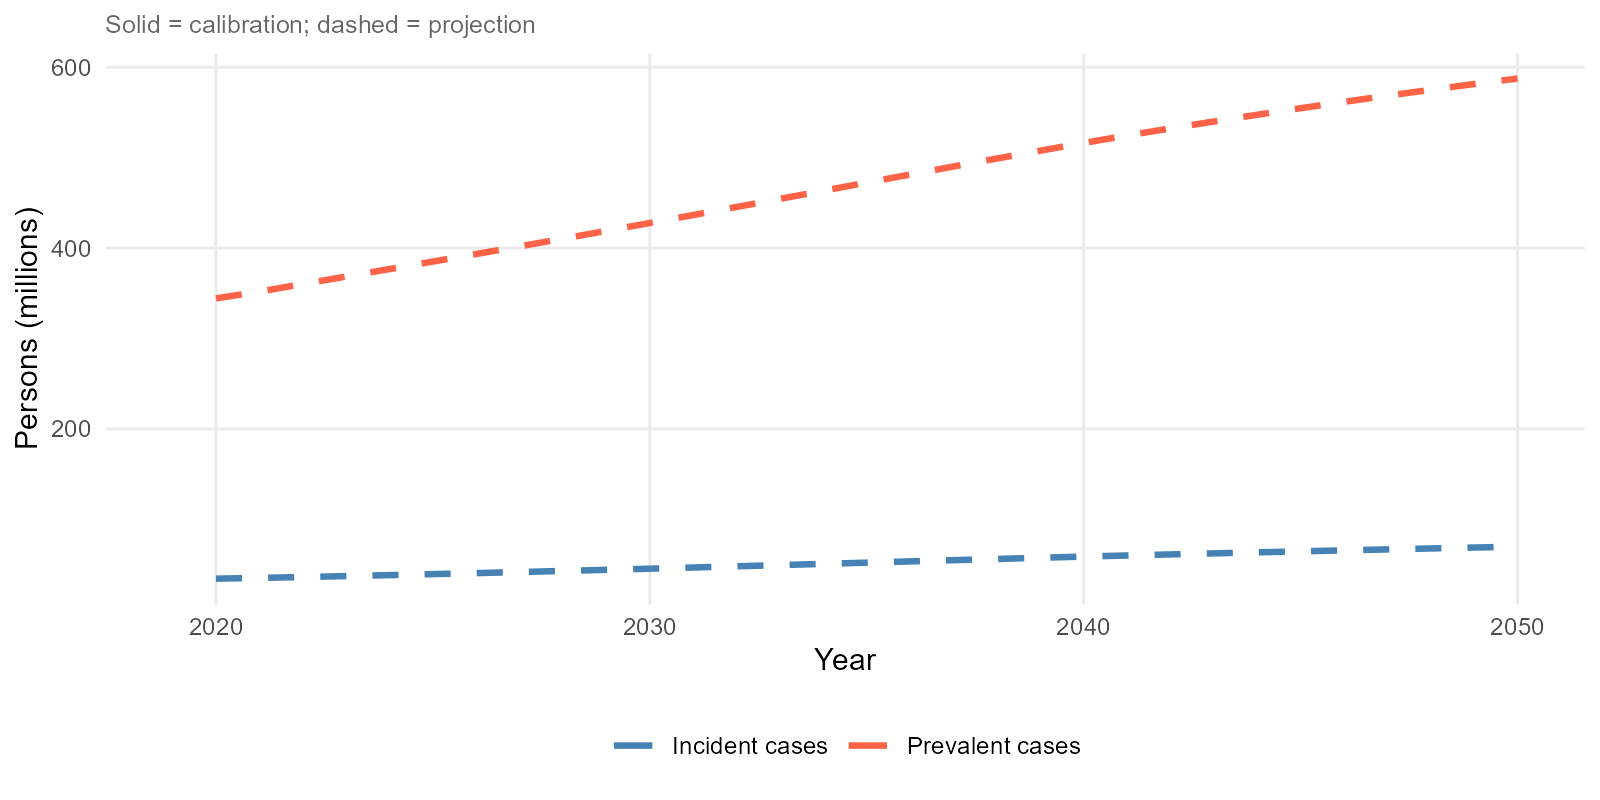
\includegraphics[width=\linewidth]{../../output/slides/sl_fig_baseline_trend} \end{center}

\footnotesize Incident and prevalent CVD cases 2019--2050; solid =
calibration, dashed = projection.
\end{frame}

\begin{frame}{Age-Standardised CVD Mortality Rate}
\phantomsection\label{age-standardised-cvd-mortality-rate}
\begin{center}\includegraphics[width=\linewidth]{aim1_executive_slides_files/figure-beamer/fig-asmr-1} \end{center}
\end{frame}

\begin{frame}{Summary: Cumulative Deaths Averted, 2026--2050}
\phantomsection\label{summary-cumulative-deaths-averted-20262050}
\begin{table}[!h]
\centering\begingroup\fontsize{9}{11}\selectfont

\resizebox{\ifdim\width>\linewidth\linewidth\else\width\fi}{!}{
\begin{tabular}{llll}
\toprule
Scenario & Cumulative (M) & Avg./year (M) & \% of BAU deaths\\
\midrule
HTN Control (No Diabetes) & 20.2 M & 0.8 M & 2.9\%\\
HTN Control (Diabetes) & 26.7 M & 1.1 M & 3.9\%\\
Improved Statin Uptake & 21.2 M & 0.8 M & 3.1\%\\
\cellcolor[HTML]{6a3d9a}{\textcolor{white}{\textbf{All Interventions}}} & \cellcolor[HTML]{6a3d9a}{\textcolor{white}{\textbf{35.3 M}}} & \cellcolor[HTML]{6a3d9a}{\textcolor{white}{\textbf{1.4 M}}} & \cellcolor[HTML]{6a3d9a}{\textcolor{white}{\textbf{5.1\%}}}\\
\bottomrule
\end{tabular}}
\endgroup{}
\end{table}

\begin{exampleblock}{Headline}
\textbf{All Interventions}: \textbf{35.3 million deaths averted} globally, 2026--2050 ($\approx$ 1.4 M/year).
\end{exampleblock}
\end{frame}

\begin{frame}{Annual Deaths Averted Over Time}
\phantomsection\label{annual-deaths-averted-over-time}
\begin{center}\includegraphics[width=\linewidth]{aim1_executive_slides_files/figure-beamer/fig-deaths-averted-1} \end{center}

\footnotesize Cumulative deaths averted per intervention relative to
business-as-usual.
\end{frame}

\begin{frame}{Cumulative Deaths Averted Over Time}
\phantomsection\label{cumulative-deaths-averted-over-time}
\begin{center}\includegraphics[width=\linewidth]{aim1_executive_slides_files/figure-beamer/fig-cum-averted-1} \end{center}

\footnotesize Cumulative deaths averted per intervention relative to
business-as-usual.
\end{frame}

\begin{frame}{Deaths Averted by Cause of Death}
\phantomsection\label{deaths-averted-by-cause-of-death}
\begin{center}\includegraphics[width=\linewidth]{aim1_executive_slides_files/figure-beamer/fig-by-cause-1} \end{center}
\end{frame}

\begin{frame}{Deaths Averted by Age Group}
\phantomsection\label{deaths-averted-by-age-group}
\begin{center}\includegraphics[width=\linewidth]{aim1_executive_slides_files/figure-beamer/fig-by-age-1} \end{center}
\end{frame}

\begin{frame}{Burden of Disease Averted: YLLs, YLDs, and DALYs}
\phantomsection\label{burden-of-disease-averted-ylls-ylds-and-dalys}
\begin{itemize}
\tightlist
\item
  DALYs averted: 450.0 M
\item
  YLLs averted: 460.9 M
\item
  YLDs averted: -10.8 M
\end{itemize}

\begin{longtable}[]{@{}
  >{\raggedright\arraybackslash}p{(\linewidth - 8\tabcolsep) * \real{0.3210}}
  >{\raggedleft\arraybackslash}p{(\linewidth - 8\tabcolsep) * \real{0.1852}}
  >{\raggedleft\arraybackslash}p{(\linewidth - 8\tabcolsep) * \real{0.1728}}
  >{\raggedleft\arraybackslash}p{(\linewidth - 8\tabcolsep) * \real{0.1605}}
  >{\raggedleft\arraybackslash}p{(\linewidth - 8\tabcolsep) * \real{0.1605}}@{}}
\toprule\noalign{}
\begin{minipage}[b]{\linewidth}\raggedright
Intervention
\end{minipage} & \begin{minipage}[b]{\linewidth}\raggedleft
Deaths averted
\end{minipage} & \begin{minipage}[b]{\linewidth}\raggedleft
DALYs averted
\end{minipage} & \begin{minipage}[b]{\linewidth}\raggedleft
YLDs averted
\end{minipage} & \begin{minipage}[b]{\linewidth}\raggedleft
YLLs averted
\end{minipage} \\
\midrule\noalign{}
\endhead
HTN Control (No Diabetes) & 19.8 M & 283.4 M & 10.7 M & 294.1 M \\
HTN Control (Diabetes) & 26.4 M & 327.8 M & 13.2 M & 341.0 M \\
Improved Statin Uptake & 21.2 M & 264.3 M & -1.8 M & 262.5 M \\
All Interventions & 35.0 M & 460.9 M & -10.8 M & 450.0 M \\
\bottomrule\noalign{}
\end{longtable}

\begin{exampleblock}{Headline}
\footnotesize
The combined WHO target package generates large health gains, with most benefits coming through avoided premature CVD deaths rather than morbidity reduction alone.
\end{exampleblock}
\end{frame}

\begin{frame}{Regional Summary}
\phantomsection\label{regional-summary}
\begin{table}[!h]
\centering\begingroup\fontsize{9}{11}\selectfont

\resizebox{\ifdim\width>\linewidth\linewidth\else\width\fi}{!}{
\begin{tabular}{llll}
\toprule
\textbf{Region} & \textbf{BAU deaths (M)} & \textbf{Averted (M)} & \textbf{\% averted}\\
\midrule
Western Pacific & 225.9 & 12.6 & 5.6\%\\
South-East Asia & 175.8 & 7.3 & 4.2\%\\
Europe & 117.2 & 5.8 & 4.9\%\\
Americas & 62.6 & 4.0 & 6.4\%\\
Eastern Mediterranean & 64.0 & 3.5 & 5.4\%\\
\addlinespace
Africa & 48.7 & 2.1 & 4.2\%\\
\bottomrule
\end{tabular}}
\endgroup{}
\end{table}

\vspace{4pt}
\begin{block}{Observation}
Absolute gains largest in high-burden regions; proportional gains reflect current coverage gaps.
\end{block}
\end{frame}

\section{Economic Value of Avoidable
Mortality}\label{economic-value-of-avoidable-mortality}

\begin{frame}{Economic Valuation: Methods at a Glance}
\phantomsection\label{economic-valuation-methods-at-a-glance}
\begin{columns}[T]
\begin{column}{0.55\textwidth}
\textbf{Two complementary metrics}
\begin{itemize}\footnotesize
  \item \textbf{Value of Statistical Life (VSL)} --- monetary value the population places on small reductions in mortality risk; transferred from a U.S.\ reference using country GNI per capita (PPP) and an income elasticity.
  \item \textbf{Value of Statistical Life Year (VSLY)} --- VSL annuitised by remaining life expectancy at the average adult age, then applied to age-specific life-years gained from deaths averted.
\end{itemize}

\medskip
\textbf{Headline framing}: VSLY is reported as a \textbf{proportion of annual income} (discounted GNI) so results are directly comparable across regions and over time.
\end{column}

\begin{column}{0.43\textwidth}
\begin{exampleblock}{Reference-case parameters}
\footnotesize
\textbf{Income elasticity (primary):} differential 0.8 (HIC) / 1.2 (LMIC), per Robinson et al.~(2019)\\
\textbf{Sensitivity:} uniform $e = 1.5$\\
\textbf{Discount rate:} 3\% (calendar-year)\\
\textbf{Income projection:} World Bank GNI (PPP), forward-projected with SSP2 GDP growth\\
\textbf{Horizon:} 2026--2050
\end{exampleblock}

\begin{block}{Methodological alignment}
\footnotesize
Approach follows \textbf{Robinson et al.\ (2019)} guidance and is consistent with recent published modelling of CVD policy benefits in World Bank’s Healthy Longevity Initiative \textit{Nature Medicine} papers (Chang et al.\ 2024; Verguet et al.\ 2024).

\end{block}
\end{column}
\end{columns}
\end{frame}

\begin{frame}{Economic Value by WHO Region (Primary, Cumulative
2026--2050)}
\phantomsection\label{economic-value-by-who-region-primary-cumulative-20262050}
\begin{exampleblock}{World: All Interventions, 2026--2050 (primary, discounted at 3\%)}
\textbf{VSLY} = \textbf{1.0\%} of annual income PPP (cumulative \textbf{\$41.5 T}).
\end{exampleblock}

\begin{table}[!h]
\centering\begingroup\fontsize{8}{10}\selectfont

\resizebox{\ifdim\width>\linewidth\linewidth\else\width\fi}{!}{
\begin{tabular}{lrr}
\toprule
\textbf{Region} & \textbf{VSLY (USD T)} & \textbf{VSLY \% GNI}\\
\midrule
Africa & \$0.6 & 0.3\%\\
Americas & \$6.8 & 0.8\%\\
Eastern Mediterranean & \$2.6 & 0.9\%\\
Europe & \$11.7 & 1.3\%\\
South-East Asia & \$4.7 & 0.7\%\\
\addlinespace
Western Pacific & \$15.1 & 1.4\%\\
\cellcolor[HTML]{2166ac}{\textcolor{white}{\textbf{World}}} & \cellcolor[HTML]{2166ac}{\textcolor{white}{\textbf{\$41.5}}} & \cellcolor[HTML]{2166ac}{\textcolor{white}{\textbf{1.0\%}}}\\
\bottomrule
\end{tabular}}
\endgroup{}
\end{table}
\end{frame}

\begin{frame}{Value of Avoidable Mortality as a Proportion of Income}
\phantomsection\label{value-of-avoidable-mortality-as-a-proportion-of-income}
\begin{center}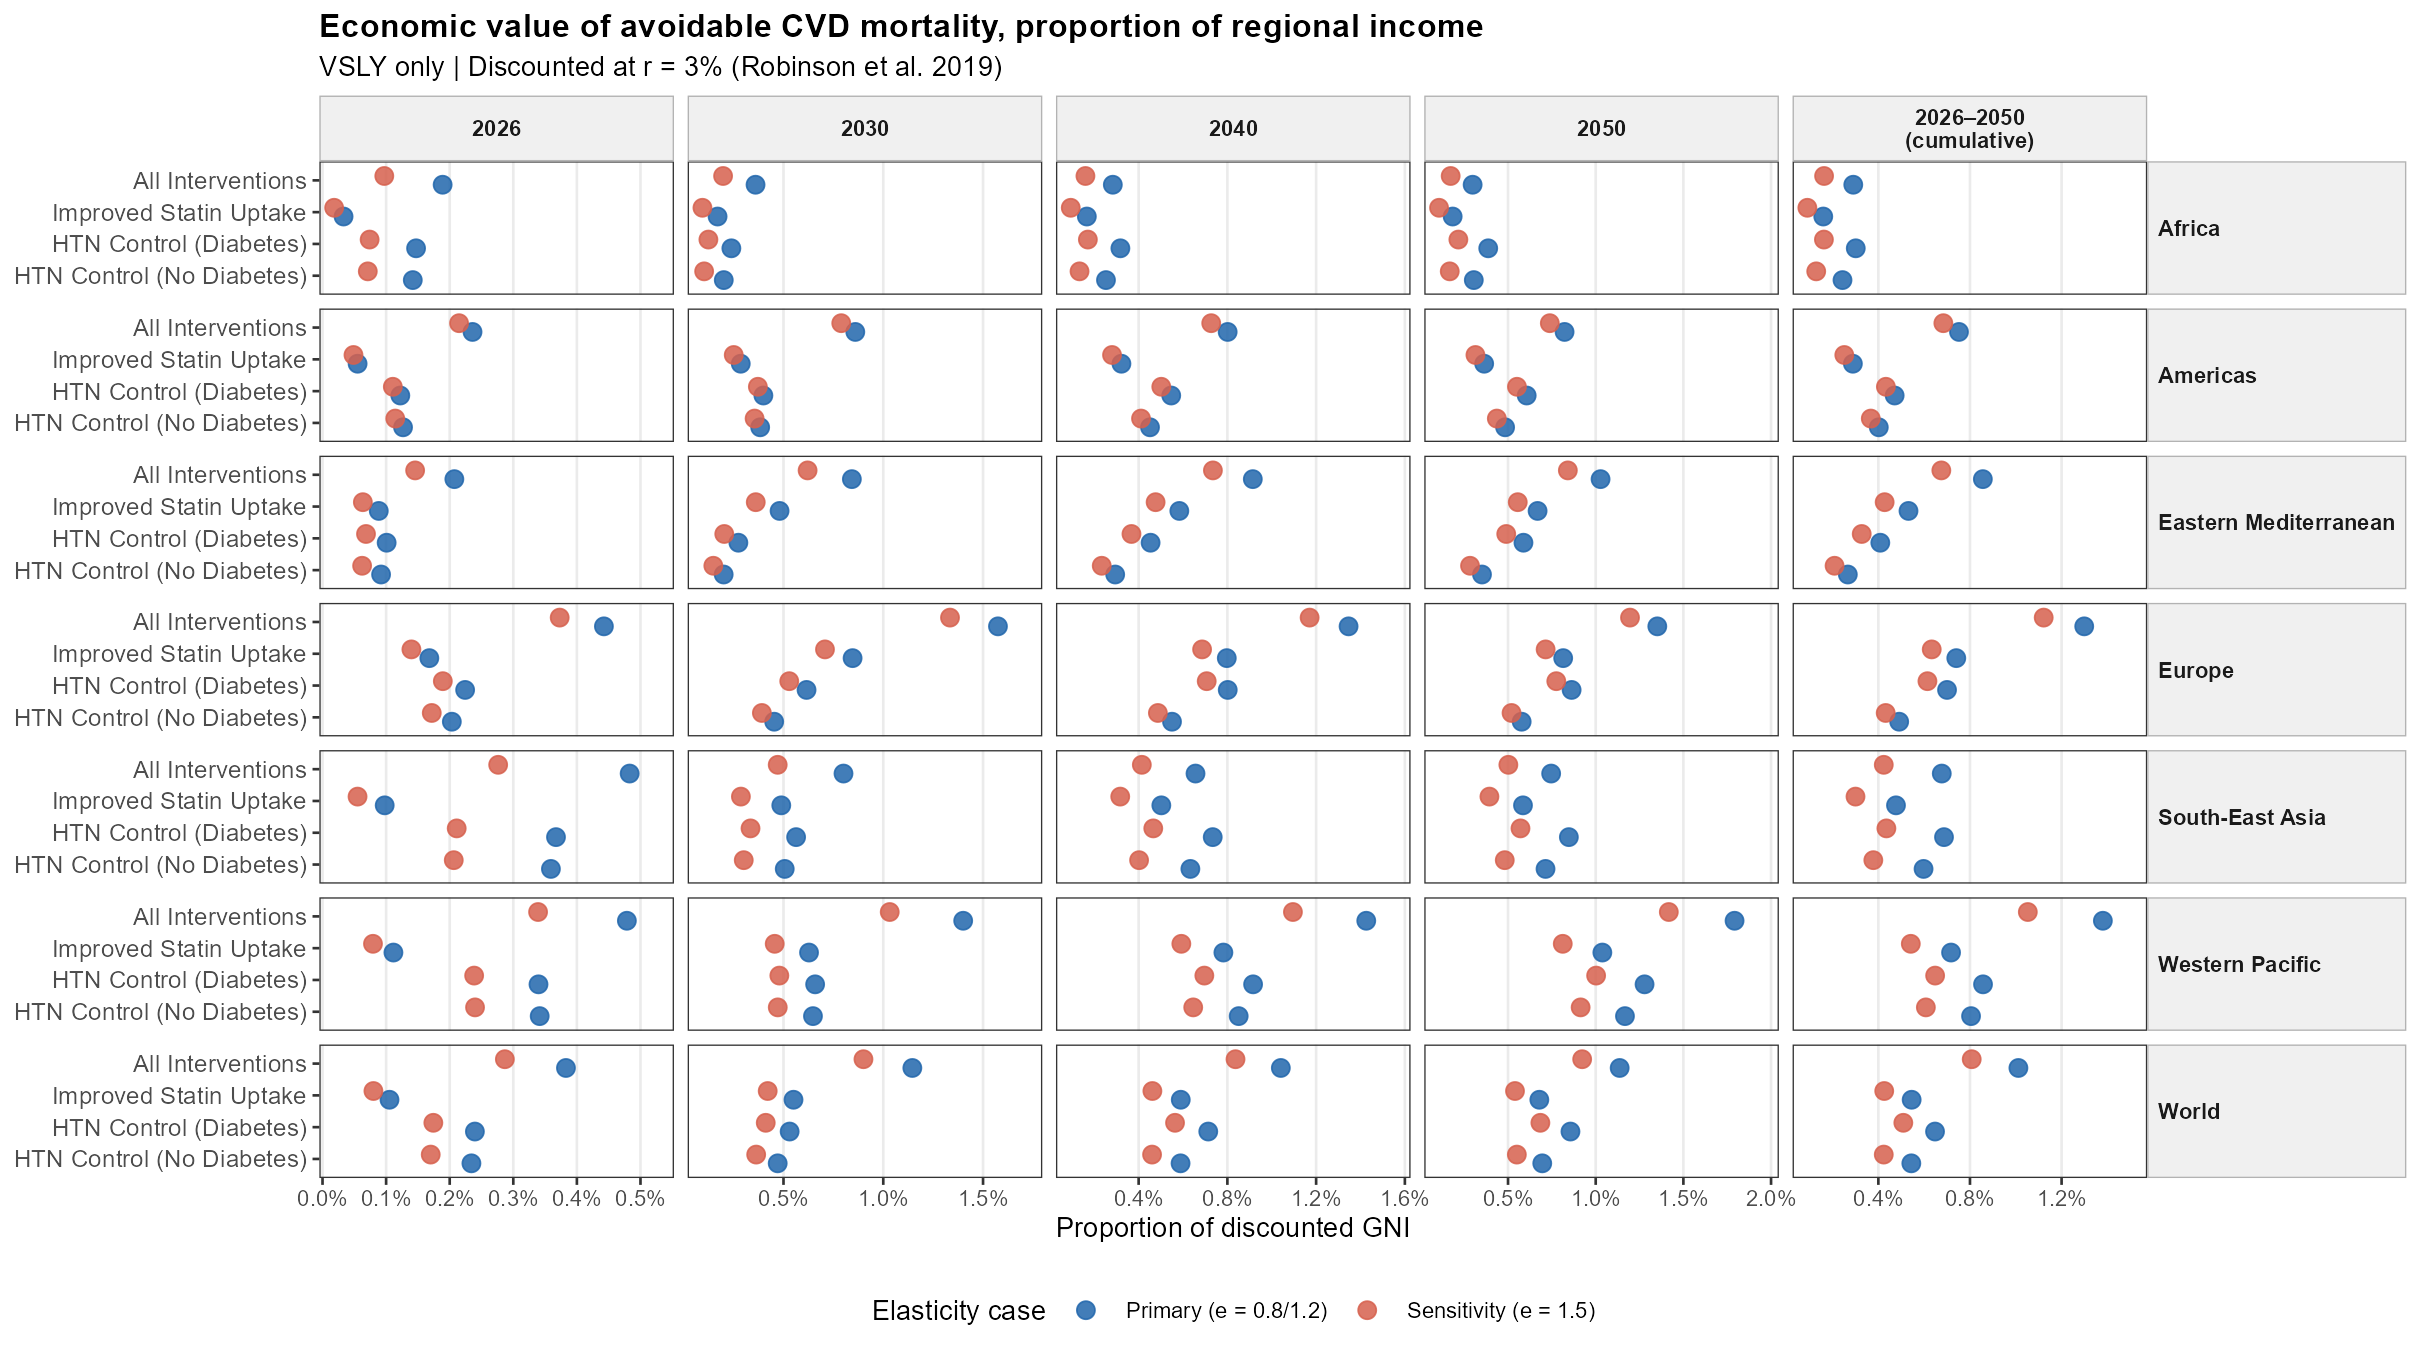
\includegraphics[width=\linewidth]{../../output/slides/sl_econ_dotplot} \end{center}

\scriptsize Dot plot: VSL (\textbullet) and VSLY (\(\blacktriangle\))
values as a proportion of discounted GNI, by WHO region \(\times\)
snapshot year and cumulative 2026--2050. Blue = primary elasticity (e =
0.8 HIC / 1.2 LMIC); red = sensitivity (uniform e = 1.5).
\end{frame}

\section{Discussion}\label{discussion}

\begin{frame}{Interpretation}
\phantomsection\label{interpretation}
\begin{columns}[T]
\begin{column}{0.55\textwidth}
\textbf{Key findings}
\begin{itemize}
  \item \textbf{All Interventions} yields largest gains: HTN control + statins are complementary
  \item \textbf{IHD} and \textbf{ischemic stroke} drive the majority of avertable deaths
  \item Gains \textbf{accelerate after 2030} as coverage compounds
  \item \textbf{Older adults (70+)} benefit most in absolute terms
  \item \textbf{Top 15 countries} account for $>$75\% of avertable burden
\end{itemize}
\end{column}
\begin{column}{0.43\textwidth}
\begin{exampleblock}{Policy Implication}
Combined WHO Targets 1 + 2 are synergistic --- neither alone captures the full benefit.
\end{exampleblock}
\vspace{6pt}
\begin{alertblock}{Uncertainty \textcolor{red!70!black}{$\bigtriangleup$}}
Sensitivity analysis to diabetes targeting assumptions and secular trends pending.
\end{alertblock}
\end{column}
\end{columns}
\end{frame}

\begin{frame}{Limitations}
\phantomsection\label{limitations}
\begin{columns}[T]
% ---------------- Left column ----------------
\begin{column}{0.48\textwidth}

\textbf{Model structure \& assumptions}
\begin{itemize}\footnotesize
  \item Stable transition rates assumed; no dynamic feedback between states
  \item Static BP distribution (log-normal): no secular trend and no endogenous updating as coverage increases
  \item No heterogeneity in adherence: newly HTN covered individuals assumed fully adherent
  \item COVID-19 excess mortality only modelled for 2020--2021; long-term effects excluded
\end{itemize}

\medskip
\textbf{Data \& parameters}
\begin{itemize}\footnotesize
  \item RCT-based effect sizes (e.g., Ettehad $\rho_{CF}$): real-world effectiveness at scale may be lower
  \item GBD 2023 uncertainty intervals not propagated
  \item Baseline $C_0$ from NCD-RisC; measurement error unquantified
  \item BP distributions rely on GBD modelling (not direct surveys in all countries)
  \item Statin coverage sparse in some LMICs; imputed from sub-regional estimates
\end{itemize}

\end{column}

% ---------------- Right column ----------------
\begin{column}{0.48\textwidth}

\textbf{Scenarios \& implementation realism}
\begin{itemize}\footnotesize
  \item Linear scale-up assumed (2026--2030); real programmes may follow non-linear trajectories
  \item No explicit health-system capacity constraints modelled
  \item Interactions with statins, diabetes care, and \alert{BP device availability} not included
\end{itemize}

\end{column}
\end{columns}
\end{frame}

\begin{frame}{Next Steps}
\phantomsection\label{next-steps}
\begin{columns}[T]
\begin{column}{0.55\textwidth}
\textbf{Analysis priorities}
\begin{enumerate}
  \item Sensitivity analysis on effect sizes, trends and coverage
  \item Add life-years gained (LYG) and DALYs as co-primary outcome
  \item Stratify by income group (World Bank)
  \item Conduct Aim 2: simulate alternative scale-up trajectories and implementation scenarios for hypertension control
\end{enumerate}
\end{column}
\begin{column}{0.43\textwidth}
\begin{alertblock}{Pending Decisions \textcolor{red!70!black}{$\bigtriangleup$}}
\begin{itemize}
  \item Journal target?
\end{itemize}
\end{alertblock}
\end{column}
\end{columns}
\end{frame}

\begin{frame}{Summary}
\phantomsection\label{summary}
\begin{block}{\textbf{1. The health gains are large and achievable}}
All Interventions: \textbf{35.3 million deaths averted} globally, 2026--2050.
\end{block}

\begin{block}{\textbf{2. HTN control + statins compound risk reduction}}
HTN control and statins have multiplicative risk reductions, producing larger combined effects.
\end{block}

\begin{block}{\textbf{3. Regional patterns reflect burden and coverage gaps}}
Absolute gains largest in high-burden regions; proportional gains reflect current coverage gaps.
\end{block}

\begin{exampleblock}{\textbf{4. The economic value rivals annual income itself}}
World, All Interventions, 2026--2050: avoidable CVD mortality is worth \textbf{1.0\%\ of annual income} (VSLY, cumulative \textbf{\$41.5 T}, discounted at 3\%).
\end{exampleblock}

\vspace{6pt}
\begin{center}
\textit{Meeting WHO 2030 CVD targets is not just aspirational --- it is quantifiably lifesaving \emph{and} economically transformative.}
\end{center}
\end{frame}

\section{Appendix}\label{appendix}

\begin{frame}{Notation: Core Model}
\phantomsection\label{notation-core-model}
\begin{center}{\small
\begin{tabular}{ll}
\toprule
Symbol & Description \\
\midrule
\multicolumn{2}{l}{\textit{Core state-transition model}} \\
$a, s, c, t, \ell$ & Age, sex, cause, year, location \\
$W, K, D$ & Well, Sick, Dead populations \\
$IR_{a,s,c}$, $CF_{a,s,c}$ & Baseline incidence \& case-fatality rates \\
$\varepsilon_{IR,j}$, $\varepsilon_{CF,j}$ & Multiplicative effect ratios for intervention $j$ \\
$BG.mx$, $BG.mx.all$ & Cause-specific \& all-cause background mortality \\
$covid.mx$ & COVID-19 mortality (2020--2021 only) \\
\bottomrule
\end{tabular}
}\end{center}
\end{frame}

\begin{frame}{Notation: HTN Control}
\phantomsection\label{notation-htn-control}
\begin{center}{\small
\begin{tabular}{ll}
\toprule
Symbol & Description \\
\multicolumn{2}{l}{\textit{HTN control (general \& diabetes subgroup)}} \\
$C_0$, $C_t$, $C_{\text{target}}$ & Baseline, time-$t$, and target control rates \\
$\Delta C_{\text{target}}$, $\Delta C_{\text{increment}}$ & Total \& time-varying incremental coverage \\
$C_{\text{agg}}^{\Delta}$ & Population-weighted incremental coverage (hypertensive bins) \\
$P(\text{BP}_{\text{cat}})$ & BP category population distribution (8 bins) \\
$RR_{\text{GBD}}$ & GBD relative risk per 10 mmHg SBP increase \\
$\alpha_{\text{inc}}$ & Incidence normalization factor \\
$E_{D}$, $E_{N}$ & Ettehad effect sizes (diabetes, no-diabetes subgroups) \\
$e_{g,t}$ & Baseline-adjusted incremental effect for subgroup $g\in\{N,D\}$ \\
$w_{D}$ & Diabetes share among hypertensives ($=P(D\mid H)$, mixture weight) \\
$c_N$, $c_D$ & Baseline control without / with diabetes ($c_D - c_N = 0.15$) \\
$\rho_{CF,c}$ & CF reduction factor per unit incremental coverage \\
$T_{\text{start}}$, $T_{\text{end}}$ & Scale-up start (2026) \& end (2030) \\
\bottomrule
\end{tabular}
}\end{center}
\end{frame}

\begin{frame}{Notation: Statins \& Combined Effects}
\phantomsection\label{notation-statins-combined-effects}
\begin{center}{\small
\begin{tabular}{ll}
\toprule
Symbol & Description \\
\midrule
\multicolumn{2}{l}{\textit{Statin therapy}} \\
$U_{0,\ell}$, $U_{\text{target}}$ & Baseline \& target statin coverage \\
$\Delta U(t,\ell)$ & Incremental statin coverage above $U_{0,\ell}$ at time $t$ \\
$T_{\text{stat,start}}$, $T_{\text{stat,end}}$ & Statin scale-up start (2026) \& end years \\
$RR^{IR}_c$, $RR^{CF}_c$ & Trial-based RRs for incidence \& case fatality \\
$\delta^{IR}_c$, $\delta^{CF}_c$ & Risk reductions $= 1 - RR$ \\
$AF_{c,\ell}$ & Cause- \& location-specific attributable fraction (incidence only) \\
$\psi_{\text{athero}}$ & Atherosclerotic fraction of ischemic stroke ($= 0.60$) \\
$E^{IR}_{c,\ell}(t)$, $E^{CF}_{c,\ell}(t)$ & Incremental effect sizes for $IR$ and $CF$ \\
\bottomrule
\end{tabular}
}\end{center}
\end{frame}

\begin{frame}{HTN Intervention Module: 9-Step Pipeline}
\phantomsection\label{htn-intervention-module-9-step-pipeline}
\begin{table}[!h]
\centering\begingroup\fontsize{7.5}{9.5}\selectfont

\begin{tabular}{>{\centering\arraybackslash}p{0.5cm}>{\raggedright\arraybackslash}p{9.5cm}>{\raggedright\arraybackslash}p{2.8cm}}
\toprule
 & Action & Output\\
\midrule
\textbf{\cellcolor{gray!10}{1}} & \cellcolor{gray!10}{Baseline BP distribution $P(\text{BP}_{\text{cat}})$ without treatment (rx$\,=\,0$)} & \em{\cellcolor{gray!10}{$P(\text{BP}_{\text{cat}}\,|\,a,s,t)$}}\\
\textbf{2} & GBD relative risks per 10 mmHg SBP $\to$ bin-specific incidence $IR_{\text{bin}}$ & \em{$IR_{\text{bin}}$}\\
\textbf{\cellcolor{gray!10}{3}} & \cellcolor{gray!10}{Subgroup-specific Ettehad effect sizes $E_N, E_D$ (no-diabetes, diabetes) per BP bin $\times$ cause} & \em{\cellcolor{gray!10}{$E_{\text{trial}}$}}\\
\cellcolor[HTML]{dbeafe}{\textbf{4}} & \cellcolor[HTML]{dbeafe}{Linear coverage scale-up from $C_0$ to $C_{\text{target}}$, \textbf{starting 2026}} & \cellcolor[HTML]{dbeafe}{\em{$C_t(t,\,\text{BP}_{\text{cat}})$}}\\
\textbf{\cellcolor{gray!10}{5}} & \cellcolor{gray!10}{Coverage adjustment: $E_{\text{adj}} = E_{\text{trial}}(C_t - C_0)\,/\,(1 - E_{\text{trial}}\,C_0)$} & \em{\cellcolor{gray!10}{$E_{\text{adj}}(t)$}}\\
\addlinespace
\textbf{6} & New bin incidence: $IR_{\text{bin,new}} = IR_{\text{bin}} \times (1 - E_{\text{adj}})$ & \em{$IR_{\text{bin,new}}$}\\
\textbf{\cellcolor{gray!10}{7}} & \cellcolor{gray!10}{Aggregate: $IR_{\text{new}} = \sum IR_{\text{bin,new}} \times P(\text{BP}_{\text{cat}})$} & \em{\cellcolor{gray!10}{$IR_{\text{new}}$}}\\
\cellcolor[HTML]{d4edda}{\textbf{8}} & \cellcolor[HTML]{d4edda}{Incidence effect ratio: $\varepsilon_{IR} = IR_{\text{new}}\,/\,IR_{\text{original}}$} & \cellcolor[HTML]{d4edda}{\em{$\varepsilon_{IR}\to$ model}}\\
\cellcolor[HTML]{d4edda}{\textbf{\cellcolor{gray!10}{9}}} & \cellcolor[HTML]{d4edda}{\cellcolor{gray!10}{Case-fatality effect ratio: $\varepsilon_{CF} = 1 - \rho_{CF} \times C_{\text{agg}}^{\Delta}$}} & \cellcolor[HTML]{d4edda}{\em{\cellcolor{gray!10}{$\varepsilon_{CF}\to$ model}}}\\
\bottomrule
\end{tabular}
\endgroup{}
\end{table}

\small\textit{Blue row = intervention start (2026). Green rows = outputs passed to state-transition model.}
\end{frame}

\begin{frame}{HTN Control: Coverage Scale-Up and Key Equations}
\phantomsection\label{htn-control-coverage-scale-up-and-key-equations}
\footnotesize
\begin{columns}[T]
\begin{column}{0.48\textwidth}
\textbf{Incidence pathway}

\medskip
\textit{Step 2 --- GBD RR anchors bin incidence:}
$$IR_{\text{bin}} = \frac{RR_{\text{GBD}} \times IR}{\alpha},\quad \alpha = \sum_{\text{cat}} P_{\text{cat}}\cdot RR_{\text{GBD}}$$

\textit{Step 5 --- baseline-adjusted effect (no double-counting):}
$$E_{\text{adj}}(t) = \frac{E_{\text{trial}}\,(C_t - C_0)}{1 - E_{\text{trial}}\,C_0}$$

\textit{Steps 7--8 --- population-weighted effect ratio:}
$$\varepsilon_{IR} = \frac{\sum IR_{\text{bin,new}} \cdot P_{\text{cat}}}{IR_{\text{original}}}$$
\end{column}

\begin{column}{0.48\textwidth}
\textbf{Case fatality pathway}

\medskip
\textit{Incremental coverage above baseline:}
$$\Delta C_{\delta}(t) = \max(C_t - C_0,\;0)$$

\textit{Aggregate across hypertensive bins ($\geq$140 mmHg):}
$$C_{\text{agg}}^{\Delta} = \frac{\sum_{\geq140}\Delta C_{\delta}\cdot P_{\text{cat}}}{\sum_{\geq140} P_{\text{cat}}}$$

\textit{CF effect ratio:}
$$\varepsilon_{CF} = 1 - \rho_{CF}\times C_{\text{agg}}^{\Delta}$$

\small
\begin{tabular}{@{}lc@{}}
\toprule Cause & $\rho_{CF}$ \\ \midrule
IHD & 0.24 \\ Ischemic stroke & 0.36 \\
Hemorrhagic stroke & 0.76 \\ HHD & 0.20 \\
\bottomrule
\end{tabular}
\end{column}
\end{columns}
\end{frame}

\begin{frame}{HTN Control: Mutually Exclusive Diabetes / No-Diabetes
Subgroups}
\phantomsection\label{htn-control-mutually-exclusive-diabetes-no-diabetes-subgroups}
\footnotesize
\begin{columns}[T]
\begin{column}{0.52\textwidth}
\textbf{Two mutually exclusive, exhaustive subgroups} of the hypertensive population; each uses its own Ettehad effect size applied \emph{only} to its own share.

\medskip
\textit{Subgroup-specific incremental effect ($g \in \{N,D\}$):}
$$e_{g,t} = \frac{E_g\,(c_{g,t} - c_{g,0})}{1 - E_g\,c_{g,0}}$$

\textit{Baseline decomposition (preserves observed rate $c$):}
$$c_N = c - w_D(0.15),\qquad c_D = c + (1-w_D)(0.15)$$

\textit{Diabetes coverage scale-up toward the 0.80 ceiling:}
$$c_{D,t} = c_{D,0} + \Delta c_D\;\min\!\left[\tfrac{t-2026}{4},\,1\right]$$
\end{column}

\begin{column}{0.46\textwidth}
\textbf{Additive population mixture} ($w_D$ = diabetes share among hypertensives), \emph{one} composite BP effect --- no cross-term:
$$\varepsilon_{IR,\text{BP}} = 1 - (1-w_D)\,e_{N,t} - w_D\,e_{D,t}$$
$$\Delta c_t = (1-w_D)\,\Delta c_{N,t} + w_D\,\Delta c_{D,t}$$

\begin{exampleblock}{Why mutually exclusive?}
\small People with diabetes have higher baseline control and larger DM-specific Ettehad effects. Counting each hypertensive once (diabetes \emph{or} not) avoids double-counting and lets the two subgroup additions sum to exactly 150 million.
\end{exampleblock}

\begin{alertblock}{Combined with statins}
\small The BP composite then combines multiplicatively with the (independent) statin effect:
$$\varepsilon_{IR,\text{total}} = \varepsilon_{IR,\text{BP}} \times \varepsilon_{IR,\text{stat}}$$
\end{alertblock}
\end{column}
\end{columns}
\end{frame}

\begin{frame}{Statin Therapy: Coverage Scale-Up and Key Equations}
\phantomsection\label{statin-therapy-coverage-scale-up-and-key-equations}
\footnotesize
\begin{columns}[T]
\begin{column}{0.50\textwidth}
\textbf{Scope:} IHD \& ischemic stroke; ages $\geq 40$ only

\medskip
\textit{Incremental coverage above baseline $U_{0,\ell}$:}
$$\Delta U(t,\ell) = \Delta U_{\text{target},\ell}\;\min\!\left[\frac{t-T_{\text{stat,start}}+1}{T_{\text{stat,end}}-T_{\text{stat,start}}+1},1\right]$$
where $\Delta U_{\text{target},\ell} = \max(U_{\text{target}} - U_{0,\ell},\,0)$

\medskip
\textit{Trial-based RRs (per $\approx$1 mmol/L LDL-C reduction):}

\small
\begin{tabular}{@{}lcc@{}}
\toprule Cause & $RR^{IR}$ & $RR^{CF}$ \\ \midrule
IHD & 0.74 & 0.80 \\
Ischemic stroke & 0.80 & 0.96 \\
\bottomrule
\end{tabular}

\normalsize\medskip
\textit{Incidence (primary prevention, AF-scaled):}
$$E^{IR}_{c,\ell}(t) = \frac{AF_{c,\ell}\;\delta^{IR}_{c}\;\Delta U(t,\ell)}{1 - \delta^{IR}_{c}\;U_{0,\ell}}$$
\end{column}

\begin{column}{0.48\textwidth}
\textit{Case fatality (secondary prevention; no AF; atherosclerotic restriction for stroke):}
$$E^{CF}_{c,\ell}(t) = \begin{cases}
\dfrac{\delta^{CF}_{\text{ihd}}\;\Delta U(t,\ell)}{1 - \delta^{CF}_{\text{ihd}}\;U_{0,\ell}}, & c=\text{ihd}\\[1.2em]
\dfrac{\psi_{\text{athero}}\;\delta^{CF}_{\text{ist}}\;\Delta U(t,\ell)}{1 - \delta^{CF}_{\text{ist}}\;U_{0,\ell}}, & c=\text{istroke}
\end{cases}$$

\small $\delta^{IR}_c = 1 - RR^{IR}_c$;\quad $\psi_{\text{athero}} = 0.60$ (atherosclerotic fraction)

\normalsize\medskip
\textit{Effect ratios passed to model:}
$$\varepsilon_{IR,\text{stat}} = \begin{cases} 1 - E^{IR}_{c,\ell}(t), & a\geq40,\;c\in\{\text{ihd,istroke}\} \\ 1, & \text{otherwise} \end{cases}$$
$$\varepsilon_{CF,\text{stat}} = \begin{cases} 1 - E^{CF}_{c,\ell}(t), & a\geq40,\;c\in\{\text{ihd,istroke}\} \\ 1, & \text{otherwise} \end{cases}$$
\end{column}
\end{columns}
\end{frame}

\begin{frame}[allowframebreaks]{References}
\phantomsection\label{references}
\footnotesize

\begin{itemize}
\item
  \textbf{Ettehad D, et al.}~Blood pressure lowering for prevention of
  CVD and death. \textit{Lancet.} 2016;387:957--967.
\item
  \textbf{GBD 2023 Collaborators} (2024). Global mortality for 371
  causes. \emph{Lancet}.
\item
  \textbf{Kontis V et al.} (2019). Contributions of risk factor trends
  to cardiometabolic mortality decline. \emph{Nature Medicine}, 25,
  579--584.
\item
  \textbf{Mills KT, et al.}~Global disparities of hypertension
  prevalence and control. \textit{Circulation.} 2016;134:441--450.
\item
  \textbf{Murray CJL et al.} (2020). Global burden of 87 risk factors:
  GBD 2019. \emph{Lancet}, 396, 1223--1249.
\item
  \textbf{NCD Countdown 2030 Collaborators.}~Pathways to achieving SDG
  target 3.4. \textit{Lancet.} 2022;399:1226--1249.
\item
  \textbf{Pickersgill et al.} (2022). Modeling global 80-80-80 blood
  pressure targets and cardiovascular outcomes. In: Nature Medicine
\item
  \textbf{Pickersgill SJ et al.} (2024). Health and economic benefits of
  achieving hypertension control: a modelling study.
  \textit{Nature Medicine}.
  \url{https://www.nature.com/articles/s41591-024-03248-4}
\item
  \textbf{Robinson LA, Hammitt JK, O'Keeffe L.} (2019). Valuing
  mortality risk reductions in global benefit-cost analysis.
  \textit{Journal of Benefit-Cost Analysis} 10(S1):15--50.
\item
  \textbf{UNWPP} (2024). World Population Prospects 2024. United
  Nations.
\item
  \textbf{Watkins, D et al.} (2025). Global Impact of Single-Pill
  Combination Therapies on Cardiovascular Mortality and Events,
  2023-2050: A Modeling Study. In: JACC.
\item
  \textbf{Watkins DA et al.} (2024). Health and economic benefits of
  cardiovascular risk-factor control: a modelling study.
  \textit{Nature Medicine}.
  \url{https://www.nature.com/articles/s41591-024-03253-7}
\item
  \textbf{WHO} (2023). Global Hearts Initiative: HEARTS Technical
  Package. Geneva.
\item
  \textbf{WHO.}~Global NCD Political Declaration. Geneva: WHO; 2025.
\end{itemize}
\end{frame}

\begin{frame}
\begin{center}
\vfill
{\Large \textbf{Thank You}}\\[10pt]
{\normalsize Questions \& Discussion}\\[16pt]
\begin{beamercolorbox}[sep=6pt,center,rounded=true]{block body example}
\small Contact: David Watkins \textbar{} davidaw@uw.edu \textbar{} University of Washington
\end{beamercolorbox}
\vfill
\end{center}
\end{frame}

\end{document}
